
\section{Experiments}\label{sec:expts_all}

\begin{figure}
\centering
\subfloat[Average annotator accuracy]{
  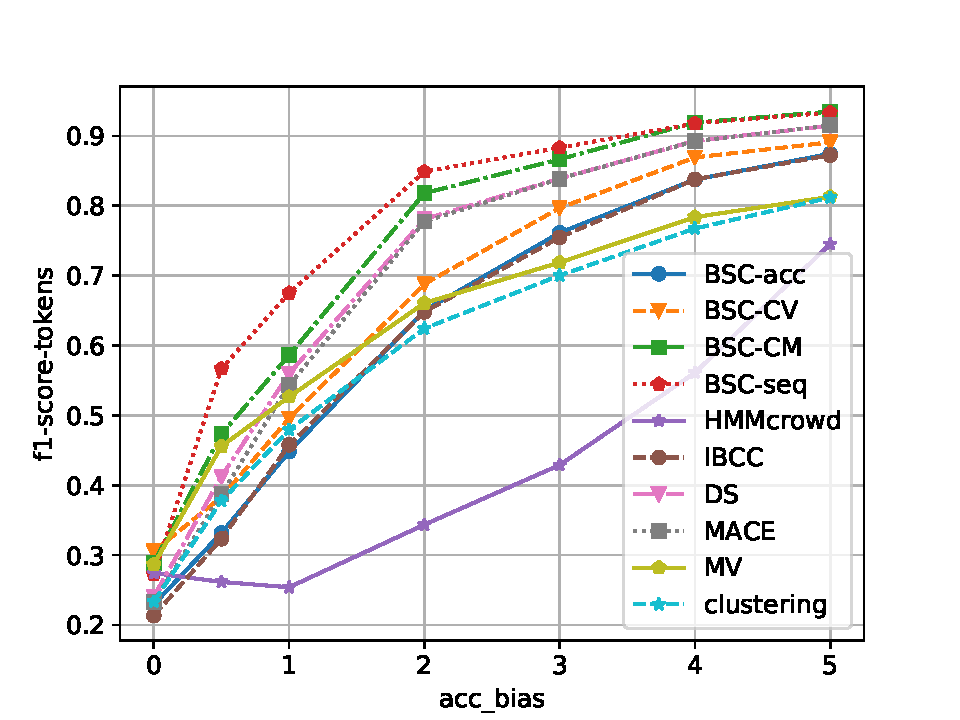
\includegraphics[width=0.9\columnwidth, clip=True, trim=10 20 40 40]{figures/synthetic/acc_bias_exp/plot_f1-score-tokens}
}\\
\subfloat[Short span bias]{
  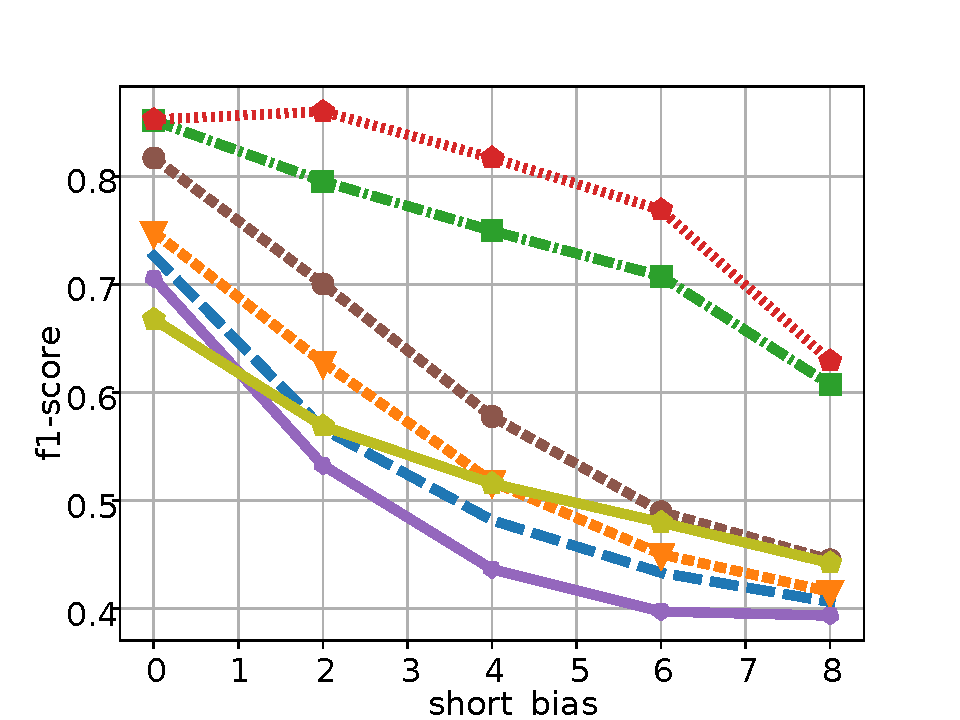
\includegraphics[width=0.9\columnwidth, clip=True, trim=10 20 40 40]{figures/synthetic/short_bias_exp/plot_f1-score-tokens}
}\\
\subfloat[Missed span bias]{
  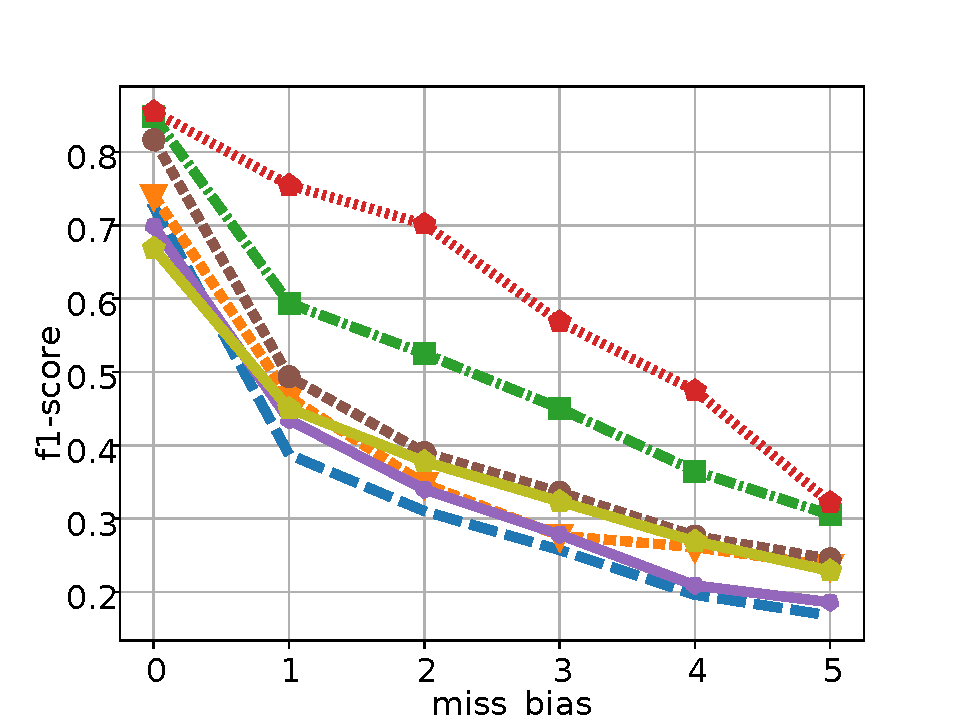
\includegraphics[width=0.9\columnwidth, clip=True, trim=10 20 40 40]{figures/synthetic/class_bias_exp/plot_f1-score-tokens}
}\\
% \subfloat[Crowd size]{
%   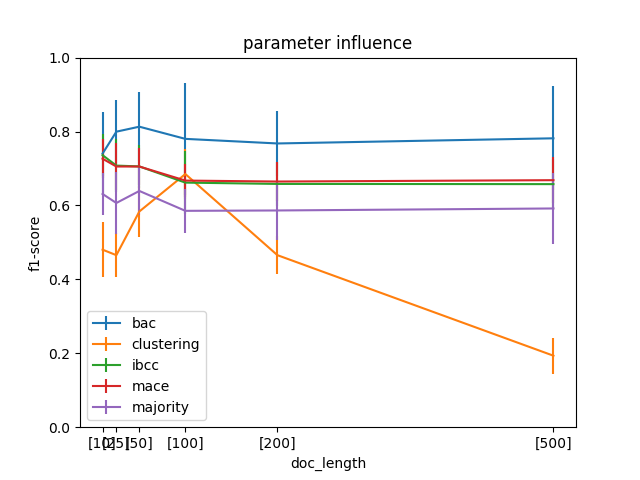
\includegraphics[width=0.2\textwidth, clip=True, trim=0 10 0 27]{figures/synthetic/acc_bias_exp/plot_f1-score.png}
% }
\subfloat[Number of good workers out of a crowd of 10, where the rest are random.]{
  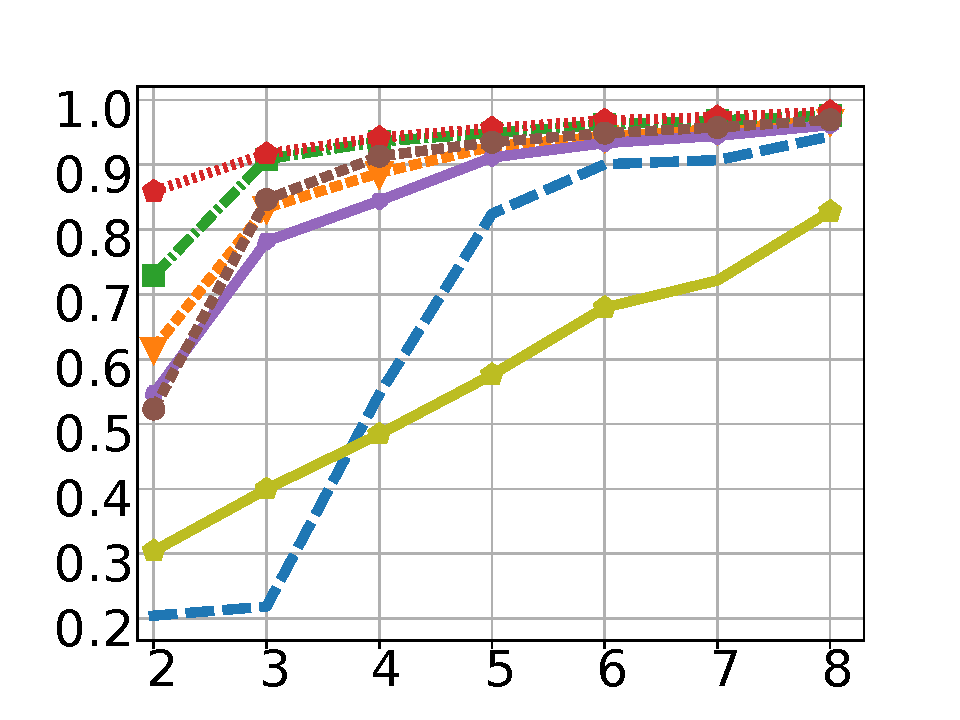
\includegraphics[width=0.9\columnwidth, clip=True, trim=10 20 40 38]{figures/synthetic/group_ratio_exp/plot_f1-score-tokens}
}
\caption{F1 scores with simulated annotators. Each plot shows the effect of varying one characteristic.}
\label{fig:simulated}
\end{figure}


We evaluate Bayesian sequence combination (BSC) against alternative methods to test 
 (a) the different annotator models described in Section \ref{sec:model},
 (b) the performance of BSC on unreliable or small training sets,
and (c) the benefits of including sequence taggers into the graphical model.
The first experiment uses simulated annotators to investigate the effects of different annotator flaws on aggregation methods. 
We then introduce two NLP datasets to 
test aggregation performance in passive and active learning scenarios, 
analyze errors,
visualize the learned annotator models,
and test LSTM 
sequence taggers~\cite{lample2016neural}
trained using our proposed method.

% We further test whether Bayesian approach facilitates more efficient active learning of sequential annotations from crowds and whether integrating the LSTM into the ensemble of annotators improves performance further.
% Our experiments consist of three tasks: (1) aggregating crowdsourced labels, (2) training the LSTM sequence tagger of Lample et al. ~\shortcite{lample2016neural} using aggregated labels, and (3) actively selecting batches of documents for crowdsourced annotation.

\subsection{Evaluated Methods}

As established non-sequential baselines, we include token-level majority voting (\emph{MV}), \emph{MACE}~\cite{hovy2013learning}, Dawid-Skene (\emph{DS})~\cite{dawid_maximum_1979} and independent Bayesian classifier combination (\emph{IBCC})~\cite{kim2012bayesian}, a Bayesian treatment of Dawid-Skene. 
We also test the sequential \emph{HMM-crowd} method \cite{nguyen2017aggregating}, which uses a combination of 
maximum \emph{a posteriori} (or smoothed maximum likelihood) estimates for a confusion vector (CV) annotator model 
and variational inference for an integrated hidden Markov model. 
%  HMM-crowd is the current state-of-the-art and allows us to compare our approach against 
%  a model without a fully Bayesian treatment. 
We also introduce a \emph{clustering} baseline,
that aggregates spans from multiple annotators by grouping them together
using kernel density estimation\cite{rosenblatt1956remarks}.

BSC is tested with each of the different annotator models described in Section \ref{sec:annomodels} and integrating different text models. 
As the default set-up, 
we integrate a simple black-box classifier
that treats all text features as conditionally independent of each other and of the sequence of labels. This set-up is tested with all annotator models.
The BSC-seq variant is also tested without a text model (\emph{notext}), 
and with an integrated LSTM~\cite{lample2016neural}, labeled \emph{BSC-seq+LSTM}.
We also use HMM-crowd and BSC-seq to produce training labels for the LSTM as a separate pre-processing step, labeled in our results as $\rightarrow$LSTM.

\subsection{Simulated Annotators}\label{sec:synexpts}

Simulated data allows us to test the effect of one  
type of error in the crowdsourced data,
while keeping other characteristics of the data constant.
We generate crowds of 10 annotators for four experiments, which  
test the effect of varying
(a) average annotator accuracy,
(b) short span bias, i.e. the probability of not including the last tokens in a span, 
(c) missed span bias, i.e. the probability of missing a span entirely,
and (d) the ratio of good to uninformative annotators in the crowd.
We simulate annotators using the generative model of BSC-seq, 
drawing annotator labeling probabilities from Dirichlet distributions. 
%given the ground truth label and the annotator's previous label.
By default, Dirichlet parameters corresponding to incorrect answers are 1,
those for correct answers are 2.5, and disallowed transitions (O$\rightarrow$I) are close to 0. 
We then change the parameters of these Dirichlet distributions 
to obtain the variations described above. 
We repeat each experiment 25 times, in each case generating 25 documents of 100 tokens each. 

Figure \ref{fig:simulated} shows the F1-scores for our tested methods. 
Where annotator accuracy is high, majority voting and clustering are less accurate than  methods that model individual annotator behavior, although the difference decreases as we introduce more errors.
Clustering performs better with high short span bias, 
as density estimation can compensate for short spans but may over-estimate
those of the correct length.
% miss bias and low average annotator accuracy, suggesting that clustering-based approaches may be worth considering in future work on span aggregation.
Among the BSC variants, performance increases with the complexity of the annotator model, from BSC-acc to BSC-seq,
suggesting that this richer model can be successfully learned on a small dataset. 
There are some benefits for the Bayesian approaches, IBCC and BSC-CV, over the similar  models, DS and HMM-crowd, respectively, in handling all four types of annotator error.
% low annotator accuracy, crowds with few good workers, short span bias and some degree of missed span bias.
%MACE mostly performs only slightly better than majority vote.
%, its spammer model
%handles short span bias and missed span bias relatively well. 

\begin{table*}
\small
\begin{tabular}{| l || r | r | r | r | r || r | r || l | r | r | r |} \hline
Dataset & \multicolumn{3}{c|}{Docs} & Sent & Tokens & \multicolumn{2}{c||}{Workers} & Span & Gold & \multicolumn{2}{c|}{Span length}  \\
 & total & gold & crowd & -ences & & total & /doc & type & spans & mean & std.  \\
\hline
NER & 1393 & 1393 & 415 & 6503 & 179323  & 47 & 4.9 & PER & 6282 & 1.19 & 0.49 \\
       & & & & & & &  & LOC  & 6482 & 1.73 & 0.57\\
       & & & & & & & & ORG  & 5789 & 1.55 & 0.92\\
       & & & & & & & & MISC & 3059 & 1.44 & 0.80\\ \hline
PICO & 4740 & 191 & 4740 & 9480 & 1424721 & 312 & 6.0 & population & 700 & 7.74 & 7.38  \\ \hline
\end{tabular}
\label{tab:datasets}
\caption{Numbers of documents, spans, annotators, tokens and sentences for our test datasets.}
\end{table*}


\subsection{Crowdsourced Datasets}\label{sec:expts}

We use two datasets containing both crowdsourced and gold sequential annotations. 
The CoNLL 2003 named-entity recognition dataset~\cite{tjong2003introduction},
\emph{NER}, contains gold labels for four named entity categories (PER, LOC, ORG, MISC),
with crowdsourced labels provided by \cite{rodrigues2014sequence}.
\emph{PICO}~\cite{nguyen2017aggregating}, 
consists of medical paper abstracts that have been annotated by a crowd to indicate text spans that identify the population enrolled in a clinical trial. 
Further information about the datasets is shown in Table \ref{tab:datasets}. Note that NER spans are typically much shorter than those in PICO.

\subsection{Evaluation Metrics}

For NER we use the CoNLL 2003 F1-score, which considers only exact span matches %(type, start and end) 
to be correct. 
%This measure is intuitive because complete named entities must be marked to be of value. 
For PICO, we use the relaxed F1-measure~\cite{nguyen2017aggregating}, which counts the matching fractions of spans when computing precision and recall.
Since the spans in PICO are longer than those of NER, partial matches may still contain much of the required information. 
%We additionally compute the root mean squared error in the span lengths, i.e. the difference between the  % actually it's not quite that. We computed the difference in mean span lengths. This is already captured by F1 score for pico and better described by the span-level-precision and recall. Our metric might be more if we didn't take the absolute so we could see if spans were often too long or too short.
We also compute the cross entropy error (\emph{CEE}) at the level of tokens
to compare the probability estimates produced by aggregation methods, which are useful for decision-making tasks such as active learning.

\subsection{Aggregating Crowdsourced Labels}\label{sec:task1}
\begin{table*}
\small
\nprounddigits{1}
\npdecimalsign{.}
\begin{tabularx}{\textwidth}{| p{1.9cm} h n{2}{1} | n{2}{1} | n{2}{1} | n{2}{1} h Y | Y  | Y  ?  n{2}{1} | n{2}{1} | n{2}{1} | n{2}{1} h Y  | Y  | Y ?}
\hline
%NER & \multicolumn{3}{|l|}{Span-level metrics}                     & \multicolumn{2}{|l|}{Token-level metrics} & Hyper.\\ \hline 
& \multicolumn{4}{l}{NER} & \multicolumn{3}{l?}{Hyperparams.} & \multicolumn{4}{l}{PICO} & \multicolumn{3}{l?}{Hyperparams.} \\ \hline
& \text{Prec.} &  \text{Rec.} & \text{F1} & \text{CEE} & $\beta_0$ & $\gamma_0$ & $\alpha_0$ & \text{Prec.} & \text{Rec.} & \text{F1} & \text{CEE} & $\beta_0$ & $\gamma_0$ & $\alpha_0$ \\ \hline

Best worker & 76.4 & 60.1 & 67.3 & %69.1 & .8521 & 
17.13  & & & &
64.8 & 53.2 & 58.5 & 17.03 & & & \\
Worst worker & 55.7 & 26.5 & 35.9 & %43.5 & .6924 & 
31.94  & & & & 
50.7 & 52.9 & 51.7 & 40.96 & & &\\ \hline

MV & 79.9 & 55.3 & 65.4 & %69.2 & .9422 & 
6.24  & & & & 82.5 & 52.8 & 64.3 & %76.4 & .923 &
 2.55  & & & \\ 
%MV$\rightarrow$LSTM & 81.2 & 58.7 & 68.1 & %71.0 & .8447 & 
%16.30 & 2 & \\ 
MACE & 74.4 & 66.0 & 70.0 & 1.01 &  .1 & .1 & 0  & 25.4 & 84.1 & 39.0 &% 44.3 & .840 &
 58.23 & .1 & .1 & 0 %72.5 & .8300 & 
\\ 
DS & 79.0 & 70.4 & 74.4 & %76.9 & .9516 & 
2.84 & & & & 71.3 & 66.3 & 68.7 &% \textbf{79.3} & .934 &
 0.44 & & & \\ 
IBCC & 79.0 & 70.4 & 74.4 & %77.1 & .9550 & 
{\npboldmath} 0.49 & .1 & 1 & .1 & 72.1 & 66.0 & 68.9 & %\textbf{79.3} & .935 & 
{\npboldmath} 0.27 & .1 & 10 & 10\\ 
%IBCC$\rightarrow$LSTM & 79.8 & 67.6 & 73.2 & %74.2 & .9040 & 
%14.01 & 86 & .1, 1, .1 \\ 
\hline

HMM-crowd & 80.5 & 69.4 & 74.6 & %77.0 & .9762 & 
1.04 & 0 & .1 & 0 & 76.5 & 66.2 & 71.0 & %77.9 & \textbf{.944} & 
0.79 & 0 & .1 & 0 \\ 
%HMM-crowd$\rightarrow$LSTMp & 81.3 & 68.6 & 74.4 & %76.1 & .9887 & 
%0.25 & 134 &  \\ 
HMM-crowd$\rightarrow$LSTM & 81.8 & 69.5 & 75.2 & %77.3 & .8972 & 
12.20 & 0 & .1 & 0 & 76.5 & 66.5 & 71.2 & %78.2 & .868 & 
12.94 & 0 & .1 & 0\\ 
\hline

BSC-acc & 83.4 & 54.3 & 65.7 & %68.2 & .9610 & 
0.96 & 10 & .1 & 10 & \textbf{89.4} & 45.2 & 60.0 & %74.5 & .9069 & 
1.59 & .1 & .1 & 10 \\ 
BSC-MACE & 67.9 & 74.1 & 70.9 & %71.6 & .9658 & 
0.89 & 10 & 10 & 1 & 46.7 & 84.4 & 60.1 & %68.5 & \textbf{.944} &
 1.98 & .1 & 100 & .1\\ 
BSC-CV & 81.4 & 64.7 & 72.1 & %75.3 & .9715 & 
0.89 & 10 & 1 & 1 & 74.9 & 67.2 & 71.1 & %77.2 & .936 &
 0.84 & .1 & 1 & .1\\ 
BSC-CM & 79.9 & 72.2 & 75.8 & %77.8 & .9635 & 
1.46 & .1 & 100 & .1 & 60.1 & 78.8 & 68.2 & %74.5 & .9434 & 
1.49 & .1 & 100 & 1 \\ 
BSC-seq & 80.3 & 74.8 & 77.4 & %78.9 & .9598 & 
0.65 & .1 & 1 & 1 & 
72.9 & 77.6 & 75.1 & %57.9 & .9250 & 
1.10 & 100 & 1 & 1\\ \hline

BSC-seq-notext & 81.0 & 69.8 & 75.0 & %76.9 & .9420 & 
0.52 & .1 & 1 & 1 & 81.2 & 59.2 & 68.5 & %59.8 & .922 &
 0.73 & .1 & .1 & .1\\ \hline

%BSC-seq$\rightarrow$LSTMp & 80.3 & 74.6 & 77.3 & %78.6 & .9910 & 
%0.20 & 129 & .1, 1, 1 \\
BSC-seq$\rightarrow$LSTM & 80.2 & 75.3 & 77.7 & %79.6 & .9262 & 
11.02 & .1 & 1 & 1 & 
75.7 & 75.4 & 75.5 & %51.6 & .821 & 
25.48 & 100 & 1 & 1 \\
%BSC-seq+LSTMp & 81.2 & 75.3 & 78.1 & %79.3 & .9574 & 
%0.54 & 0 & .1, 1, 1 \\
BSC-seq +LSTM & \textbf{82.3} & \textbf{75.9} & \textbf{78.9} & %79.6 & .9513 & 
0.59 & .1 & 1 & 1 & 
78.7 & \textbf{78.6} & \textbf{78.7} & %51.9 & .934 & 
1.15 & 100 & 1 & 1 \\
\hline
\end{tabularx}
\caption{Aggregating Crowdsourced Labels: estimating true labels for documents labelled by the crowd.}
\label{tab:aggregation_results}
\npnoround
\end{table*}
\begin{figure*}
\centering
% \subfloat[BSCC-acc-IF]{
%   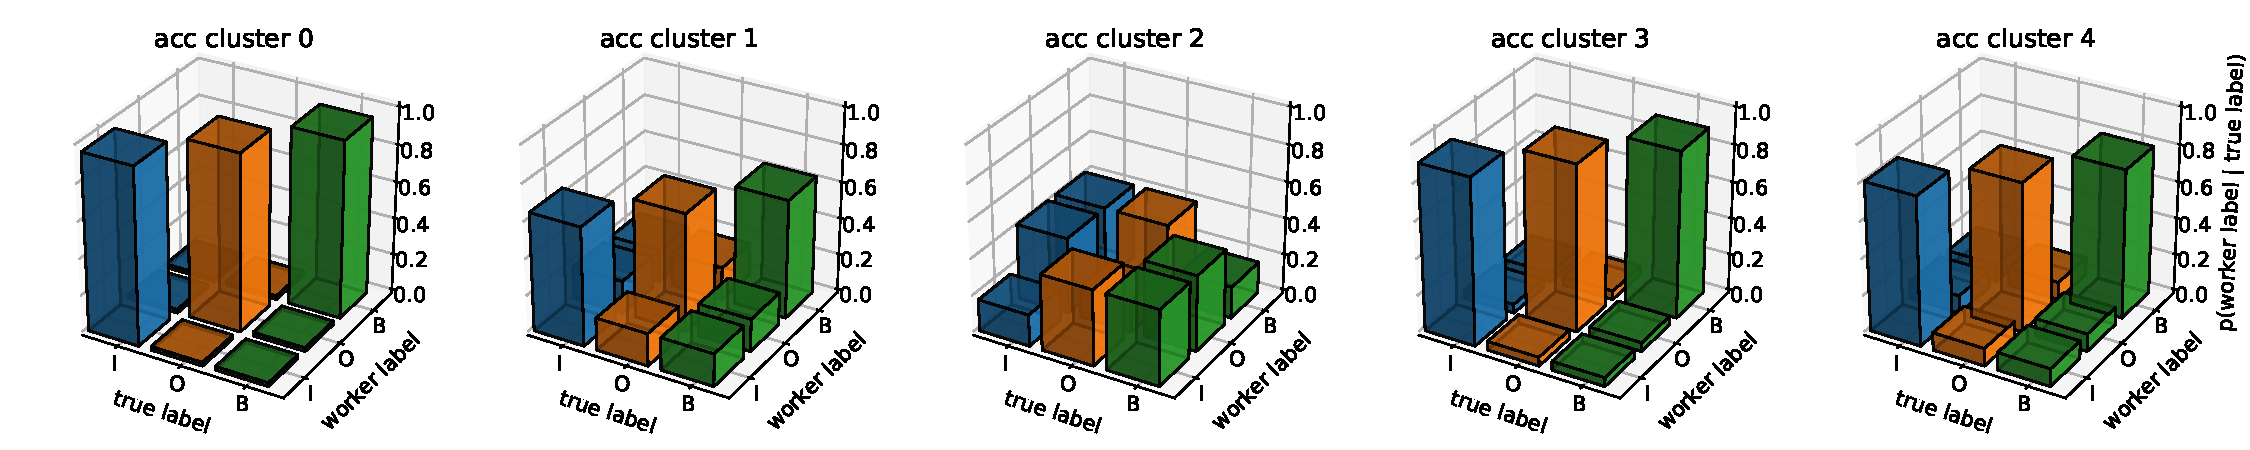
\includegraphics[width=0.9\textwidth, clip=True, trim=0 10 0 28]{figures/worker_models/acc}
% } \\
\subfloat[BSC-CV]{
  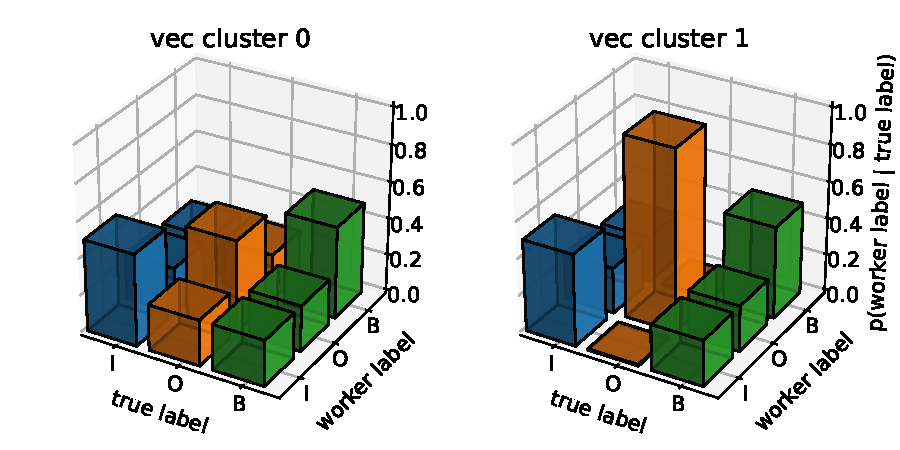
\includegraphics[width=0.7\textwidth, clip=True, trim=0 4 0 3]{figures/worker_models/vec}
} \\
% \subfloat[BSCC-MACE-IF]{
%   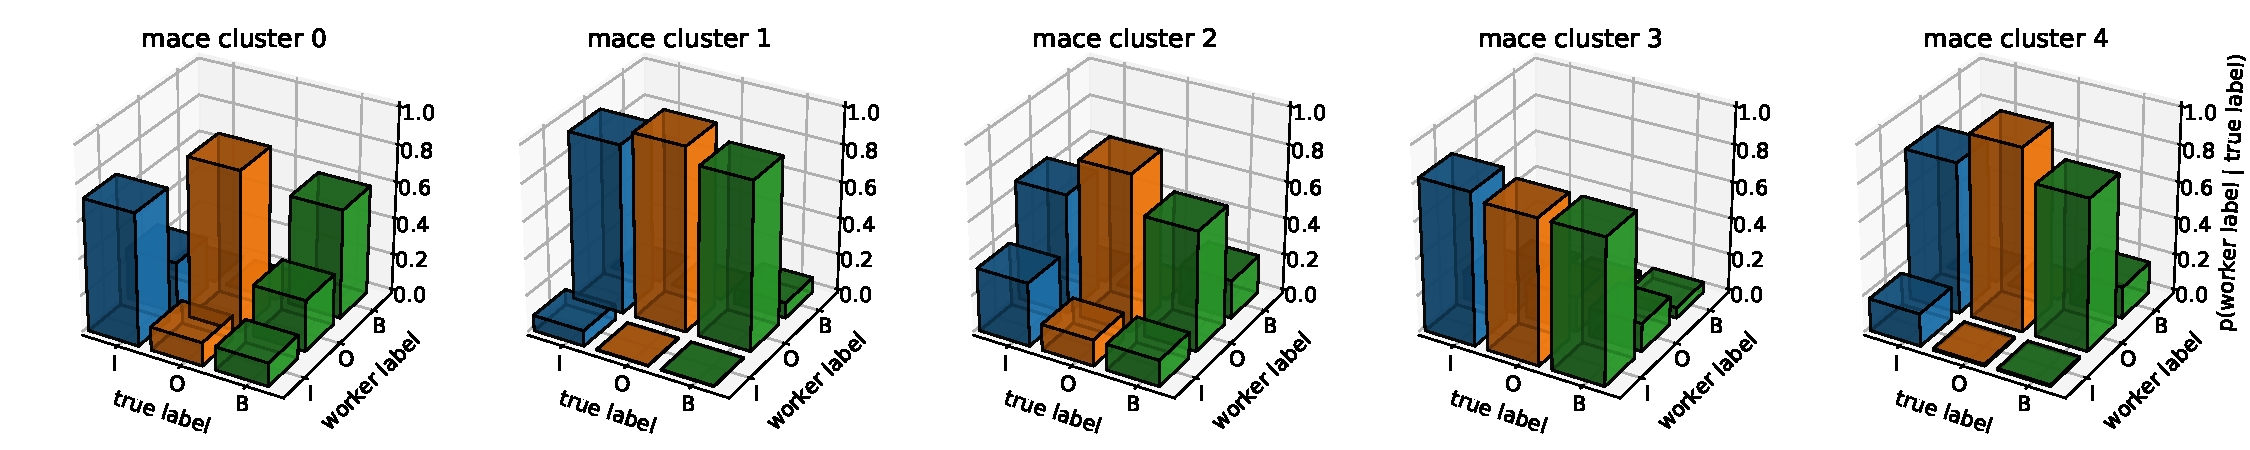
\includegraphics[width=1\textwidth, clip=True, trim=0 10 0 27]{figures/worker_models/mace}
% } \\
\subfloat[BSC-CM]{
  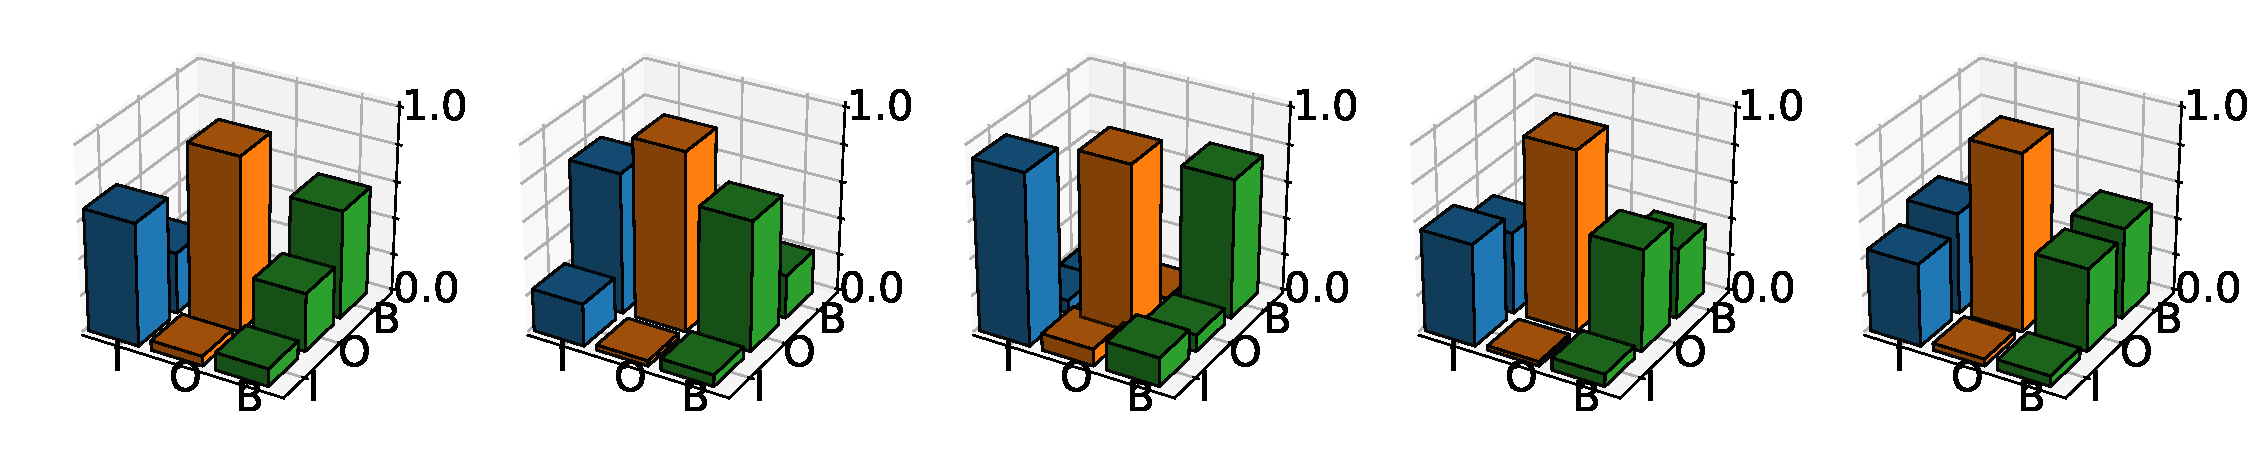
\includegraphics[width=0.7\textwidth, clip=True, trim=0 20 0 28]{figures/worker_models/ibcc}
} \\
\subfloat[BSC-seq, previous label = I]{
  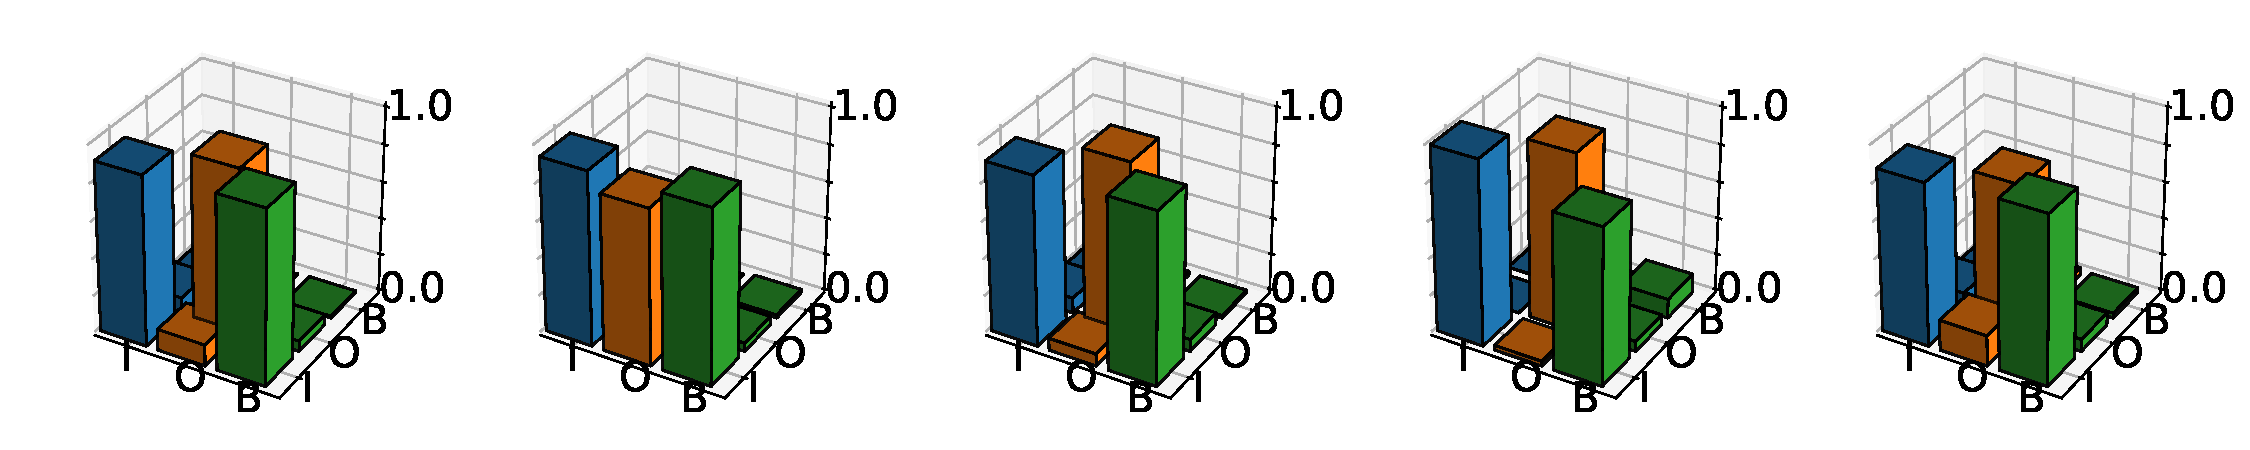
\includegraphics[width=0.7\textwidth, clip=True, trim=0 20 0 28]{figures/worker_models/seq_prev0}
} \\
\subfloat[BSC-seq, previous label = O]{
  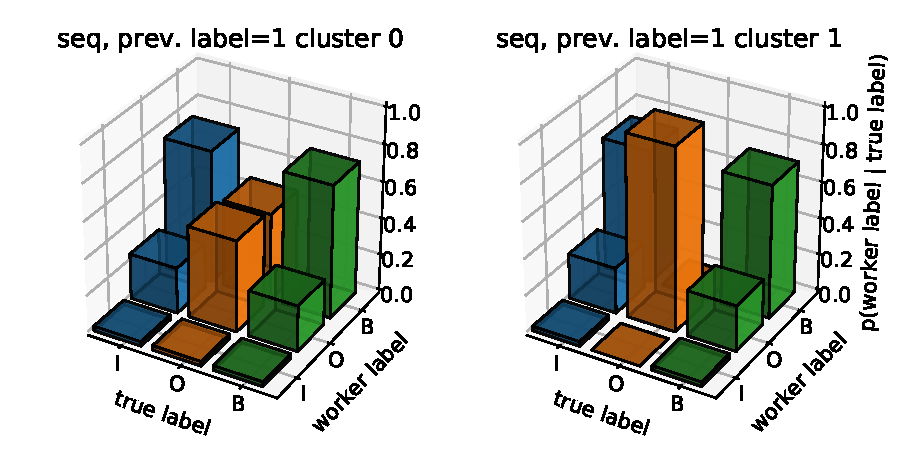
\includegraphics[width=0.7\textwidth, clip=True, trim=0 20 0 28]{figures/worker_models/seq_prev1}
} \\
\subfloat[BSC-seq, previous label = B]{
  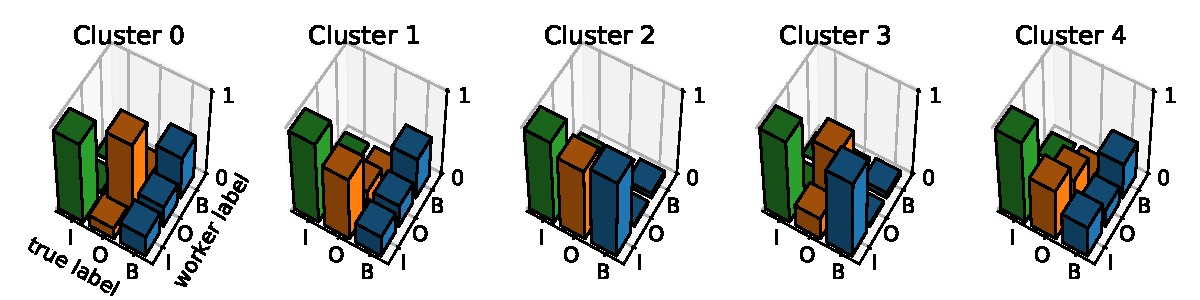
\includegraphics[width=0.7\textwidth, clip=True, trim=0 20 0 28]{figures/worker_models/seq_prev2}
} \\
\caption{Clusters of confusion matrix representations from each BSC-*** annotator model trained on PICO. 
% Show how worker representation benefits from richer model: e.g. show differences between rows in IBCC compared to acc.
% Represent all types as IBCC-confusion matrix plots. seq will need more >= 3 plots! We can focus on PICO data to make it easier to view,
% or combiner NER classes into BIO. 
% If each row corresponds to one model, we have 7 rows (2 extra for seq). 
% Each row can then show either a selection of 5 workers, or we can cluster into 5 groups.
}
\label{fig:conf_mat_clusters}
\end{figure*}
\begin{table*}
\small
\begin{tabularx}{\textwidth}{| l | X | X | X | X | X | X | X | X | X | X | X | X |}
\hline
Method & Data-set & exact match & type wrong only & partial match & mis-sing span & false +ve & late start & early start & late finish & early finish & fused spans & split span \\ \hline
MV & NER & 4307 & 304 & 228 & 1773 & 100 & 96 & 10 & 15 & 85 & 17 & 26 \\
HMM-crowd & NER & 4519 & 361 & 256 & 924 & 182 & 101 & 15 & 26 & 97 & 28 & 22 \\
BSC-CV & NER & 4431 & 275 & 243 & 1245 & 177 & 100 & 17 & 23 & 89 & 29 & 16 \\
BSC-CM & NER & 4534 & 387 & 258 & 734 & 269 & 111 & 23 & 37 & 86 & 39 & 12 \\
BSC-seq+LSTM & NER & 4581 & 351 & 261 & 564 & 195 & 93 & 42 & 33 & 85 & 39 & 17 \\
\hline
MV & PICO    & 168 & 0 & 32 & 185 & 48 & 9 & 11 & 1 & 0 & 3 & 9 \\
HMM-crowd    & PICO & 190 & 0 & 47 & 124 & 81 & 13 & 21 & 0 & 0 & 5 & 8 \\
BSC-CV       & PICO & 196 & 0 & 46 & 117 & 81 & 10 & 25 & 0 & 0 & 11 & 0 \\
BSC-CM       & PICO & 203 & 0 & 54 & 77 & 192 & 18 & 15 & 8 & 0 & 4 & 18 \\
BSC-seq+LSTM & PICO & 81 & 0 & 421 & 75 & 216 & 20 & 6 & 232 & 3 & 24 & 393 \\
\hline
\end{tabularx}
\caption{Counts of different types of span errors.}
\label{tab:error_analysis}
\end{table*}
In this task, we use the aggregation methods to combine multiple crowdsourced labels and predict the true labels for the same documents. 
For both datasets, we provide all the crowdsourced labels as input to the aggregation method. 
In both cases, we split the gold-labelled documents into 50\% validation and test sets. 
For NER, we use the split given by Nguyen et al. ~\shortcite{nguyen2017aggregating},
while for PICO, the split was not available so our results are not directly comparable to theirs.
%and they appear to have used a subset of the publicly-available dataset with on average 5 annotators per documents, rather than the 6 per document in the complete dataset.
%Note that the token-level F1-score can be skewed upwards by matching a few long spans correctly, but is useful for PICO because it shows up cases where the spans matched but the predictions were split, i.e. B is used instead of I. With non-strict entity matching, the precision and recall can be 100\% even though the prediction is split into multiple spans.
%Token-level F1-score catches this because it penalises the erroneous B tokens. With strict entity-level F1-score, the matches must be exact, so split spans would receive no credit.

To limit the number of hyperparameters to tune, we optimize only three values for BSC.
Hyperparameters of the transition matrix, $\bs\beta_j$, are set to the same value, 
$\beta_0$, except for disallowed transitions, (O$\rightarrow$I, transitions between types, e.g. I-PER$\rightarrow$I-ORG), which are set to 0.1.  
For the annotator models,
all values are set to $\alpha_0$, except for disallowed transitions, which are set to 0.1, then $\gamma_0$ is added to hyperparameters 
corresponding to correct annotations (e.g. diagonal entries in a confusion matrix).
We use validation set F1-scores to choose values from $[0.1, 1, 10, 100]$, 
training on a small subset of 250 documents for NER and 500 documents for PICO. 

The results of this task are shown in Table \ref{tab:aggregation_results}.
Although DS and IBCC do not consider sequence information nor the text itself, 
they both perform well against HMM-crowd on NER,
and BSC-CM variants on PICO. 
The improvement of DS over the results given 
by Nguyen et al. ~\shortcite{nguyen2017aggregating} may be due to implementation differences. 
Neither BSC-acc nor BSC-MACE perform strongly, with F1-scores sometimes falling below MV. 
The annotator models of BSC-CV and BSC-CM are better, although BSC-CM performs worse on PICO.
The sequential annotator model of BSC-seq performs strongly, despite
having a larger number of parameters to learn.
When the text model is removed, BSC-seq-notext performs worse than BSC-seq,
suggesting that incorporating even a simple text model provides 
a valuable boost.
% when learning the
%more complex BSC-seq model. 
Using the predictions from HMM-crowd or BSC-seq to train an LSTM produces a small improvement, but is outperformed by BSC-seq+LSTM.
% Removed the data on no. invalid spans:
% 15, 81, 81, 92, 74, 68, 0.... BSC-MACE=91
% 0, 0, 80, 30, 54, 37, 0, 40, 0000000000000, BSC\rightarrowLSTM 80

To get a deeper understanding of the key methods, we categorize the errors they make and list the
counts for each category in Table \ref{tab:error_analysis}.
All machine learning methods shown reduce the number of spans that were completely missed by majority
voting. 
BSC-seq+LSTM increases the number of exact span matches on NER, but reduces this number substantially on PICO
while increasing the number of partial matches and false postives (where no true span was present). 
This appears to be due to a larger number of split spans, where a 'B' token is inserted incorrectly inside
a span. 
Therefore, while BSC-seq outperforms the alternatives in terms of F1-score and missing spans, 
further work may be required to improve the distinction between 'B' and 'I' tokens. 

\begin{figure*}[ht]
\centering
\subfloat[NER, random sampling]{
  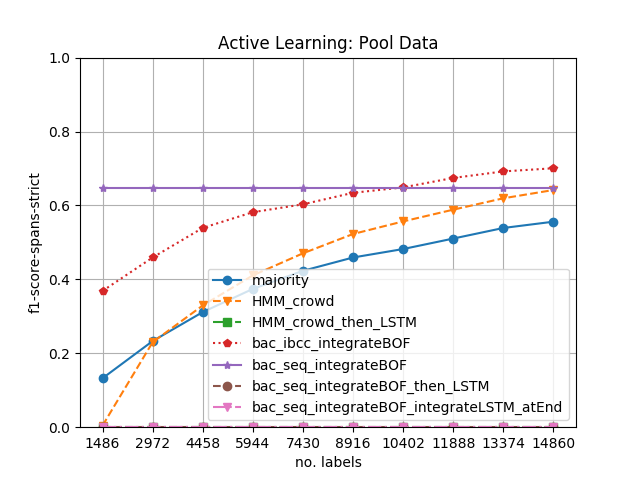
\includegraphics[width=0.9\columnwidth, clip=True, trim=12 0 0 38]{figures/NER_RAND/pool/plot_f1-score-spans-strict}
}
\subfloat[NER, active learning simulation]{
  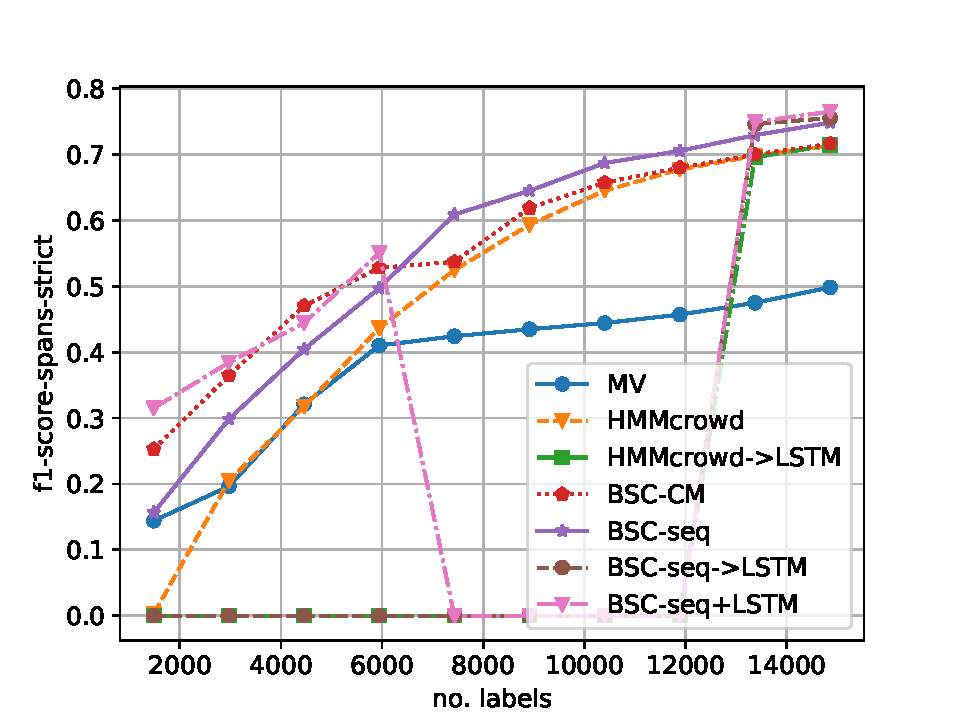
\includegraphics[width=0.9\columnwidth, clip=True, trim=12 0 0 38]{figures/NER_AL/pool/plot_f1-score-spans-strict}
}\\
\centering
\subfloat[PICO, random sampling]{
  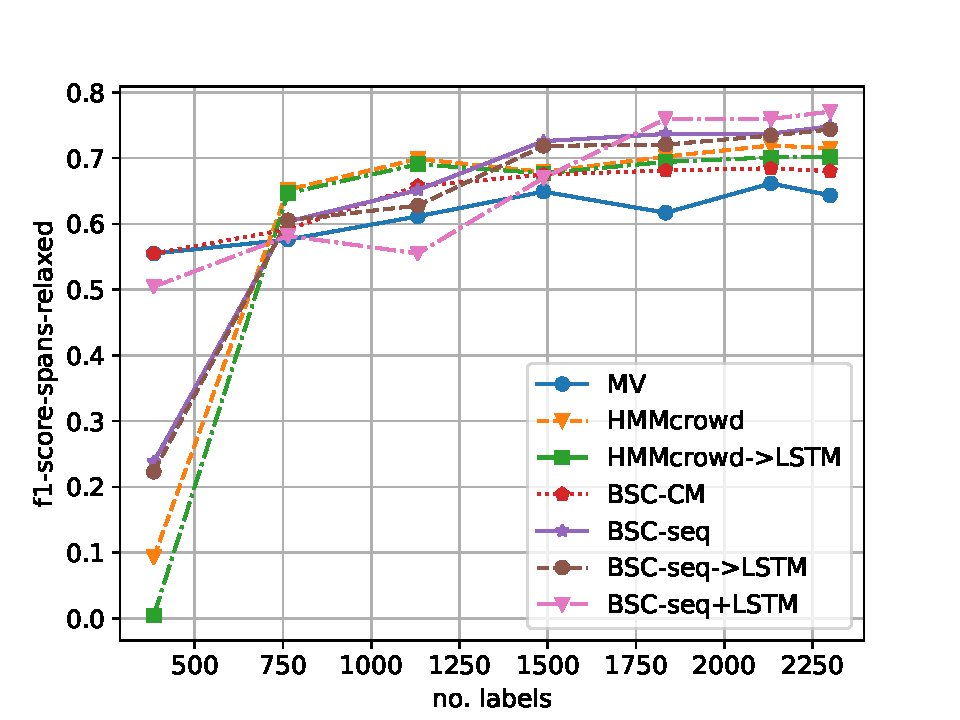
\includegraphics[width=0.9\columnwidth, clip=True, trim=12 0 0 40]{figures/PICO_RAND/pool/plot_f1-score-spans-relaxed}
}
\subfloat[PICO, active learning simulation]{
  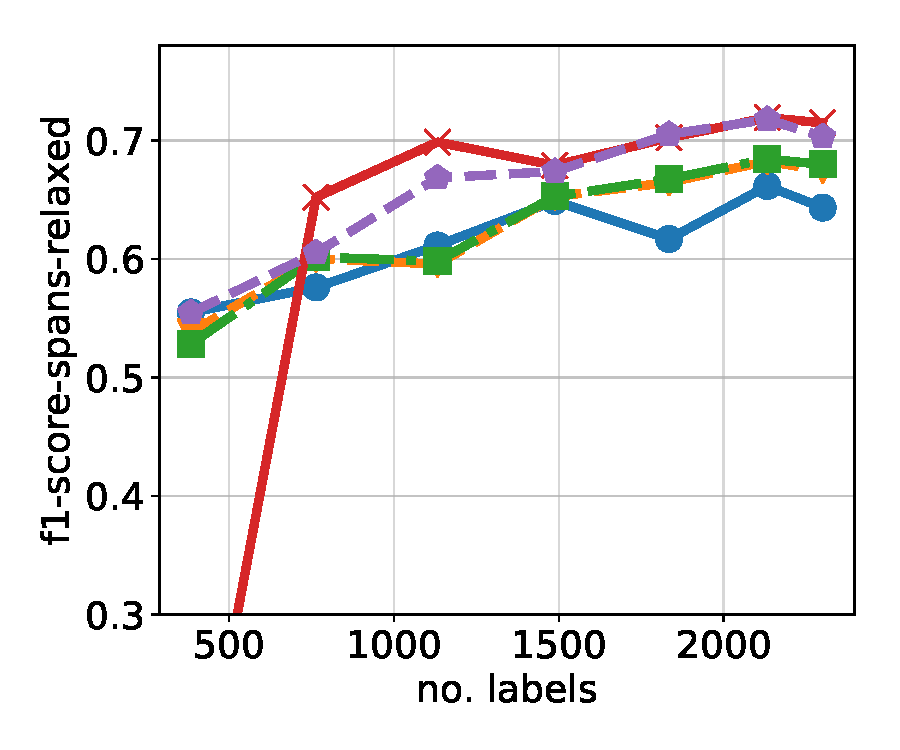
\includegraphics[width=0.9\columnwidth, clip=True, trim=12 0 0 40]{figures/PICO_AL/pool/plot_f1-score-spans-relaxed}
}
\caption{Small data subsamples: increasing span-level F1-score.
%: prediction performance after each labelled batch is received. Mean scores over 10 repeats.
}
\label{fig:alner}
\end{figure*}
Table \ref{tab:aggregation_results} shows a benefit of using the sequential annotator model over CM, CV and acc.
To understand how BSC uses the richer model in practice, we plot the learned
 annotator models for
PICO as probabilistic confusion matrices in Figure \ref{fig:conf_mat_clusters}.
To enable us to visualize the large number of annotator models, we clustered 
annotators into five groups by applying K-means to their posterior expected values.
In all clusters, BSC-CV has different heights for the diagonal entries for  B, I and O,
showing that it learns differences in accuracy for each of these label values.
BSC-CM has more distinctive clusters and the first, fourth and fifth  
have off-diagonal values with different heights for the same true label value. The second 
cluster for BSC-CM appears to encode very weakly informative labelers who usually choose 'O' regardless of the 
ground truth. 
Unlike BSC-CM, BSC-seq improved performance on PICO over BSC-CV. Its confusion matrices are
very different depending on the worker's previous annotation. 
Each column in the figure shows the confusion matrices corresponding to the same cluster of annotators. 
The first column, for example, shows
annotators with a tendency toward I$\rightarrow$I or O$\rightarrow$O transitions, while the following clusters 
indicate very different labeling behavior. The model therefore appears able to learn
distinct confusion matrices for different workers given previous labels, which supports the use of sequential
annotator models.

\subsection{Small Data and Active Learning}

We investigate the performance of the aggregation methods with smaller datasets,
and 
the effectiveness of active learning at improving performance with fewer annotations.
%improve the efficiency of the annotation process.
Two set-ups were evaluated on NER and PICO: 
the first tests our methods on random subsamples of crowdsourced data of increasing size;
the second starts with a random initial subsample,
then uses \emph{uncertainty sampling}, a well-established active learning
heuristic~\cite{settles2010active}, 
to iteratively select additional crowd labels given posterior label predictions from a model trained on the previous subset. 
We used the same random samples for all methods and repeated 
the experiments ten times with different initializations. 
\begin{table*}[t]
\small
\begin{tabularx}{\textwidth}{| l | Y | Y | Y | Y ? Y | Y | Y | Y |}
\hline
%PICO & \multicolumn{3}{|l|}{Span-level metrics (std.)}                          & \multicolumn{2}{|l|}{Token-level metrics (std.)} \\ \hline 
 & \multicolumn{4}{l?}{NER} & \multicolumn{4}{l|}{PICO}\\ \hline 
& Prec. & Recall & F1 & CEE & Prec. & Recall & F1 & CEE  \\ \hline
HMM-crowd$\rightarrow$LSTM & \textbf{78.7} & 59.0 & 67.5 &% 69.4 & .8642 &
 15.9  & \textbf{75.6} & 61.6 & 67.9 & % \textbf{76.4} & .8380 &
13.5 \\ \hline
BSC-seq$\rightarrow$LSTM & 74.3 & \textbf{62.8} & \textbf{68.1} & %69.7 & .8868 & 
15.65  & 82.3 & \textbf{66.4} & \textbf{73.5} & %58.2 & .8349 &
 19.6  \\
BSC-seq+LSTM & 72.3 & 64.2 & 68.0 &% 67.6 & .9589 &
 \textbf{0.6} & \textbf{87.4} & 57.9 & 69.7 & \textbf{0.9} \\%60.7 & 52.8 & 56.4 & 54.0 & \textbf{.899} & \textbf{0.48} & 0\\
%BCC-seq+LSTM &\\
\hline
LSTM trained on gold labels& 76.4 & 77.0 & 76.7 & %77.3 & .9563 & 
11.10 & & & & \\
\hline
\end{tabularx}
\caption{Prediction performance on test datasets with training on crowdsourced labels.}
\label{tab:prediction_results}
\end{table*}
%\begin{table}
%\small
%\begin{tabularx}{\columnwidth}{|l | Y | Y | Y |} \hline
%No. Tokens & I & O & B \\ \hline
%1486 & 0.22	& 0.978	& 0.648 \\
%14860 & 0.502	& 0.819	& 0.612 \\
%29704 & 0.695	& 0.539	& 0.533 \\ \hline
%\end{tabularx}
%\caption{Mean accuracies for the integrated LSTM learned by BSC-seq+LSTM on subsamples of NER. 
%The accuracy is the probability of correct label given the posterior expectation of the 
%sequential confusion matrix, averaged over previous label values. 
%}
%\label{tab:lstm_accs}
%\end{table}

Figure \ref{fig:alner} plots the F1 score at each iteration 
of the random sampling and active learning procedures.
BSC performs best with smaller datasets, where it may benefit from a Bayesian approach. 
Uncertainty sampling appears to have a greater improvement over random sampling on NER
after around $7000$ labels have been obtained, suggesting that a different strategy could be beneficial while
the dataset is very small. On PICO, with its smaller sample sizes, the effect of active learning is only observed
with BSC-seq+LSTM.
BSC-seq$\rightarrow$LSTM and HMM-crowd$\rightarrow$LSTM are effective on NER with smaller datasets, improving over BSC-seq and HMM-crowd methods that 
use only a simple independent text model to make predictions for unlabeled data. 
However, on PICO, they underperform BSC-seq and HMM-crowd respectively. 
BSC-seq+LSTM accounts for uncertainty in the predictions of the integrated LSTM, 
enabling it to outperform BSC-seq$\rightarrow$LSTM when active learning aquires more than $10000$ labels.
We observe that
 BSC-seq$\rightarrow$LSTM learns different values for the accuracy of the integrated LSTM depending on the true class label, even with only 1486 tokens  labeled by the crowd.

%By examining the posterior reliability model for the integrated LSTM learned by 
%, we observe that 
%Table \ref{tab:lstm_accs} shows that even for small datasets, BSC-seq+LSTM learns to account for the unreliability
%of the LSTM itself.
% The selection method and batch size could be fine-tuned for future applications -- the 
% goal of our experiment in this paper was to test the benefits of the proposed aggregation methods,
% rather than to establish a robust active learning approach.
% BSC-seq+LSTM models the reliability of the integrated LSTM. 
% Table \ref{tab:lstm_accs} summarises the accuracies learned by the model for each class label
% on the NER dataset. The differences in the inferred accuracy of the LSTM for each class shows that
% the model is able to make use

\subsection{Prediction with Crowd-Trained LSTMs}\label{sec:task2}

We compare the LSTM sequence taggers~\cite{lample2016neural}
trained by HMM-crowd and BSC-seq on test data from NER and PICO. 
For NER, we use the original CoNLL English test set~\cite{tjong2003introduction},
while for PICO, we train the aggregators on the $3,649$ documents without gold labels, 
then evaluate on the gold-labelled test data split used in Section \ref{sec:task1}.

The results in Table \ref{tab:prediction_results} show that the LSTM trained with 
BSC-seq predictions outperforms that trained using the outputs of HMM-crowd, 
the previous state-of-the-art~\cite{nguyen2017aggregating}.
 However, while BSC-seq+LSTM also outperforms
HMM-crowd$\rightarrow$LSTM and produces the lowest cross entropy error, 
its F1-scores are lower than those of BSC-seq$\rightarrow$LSTM. 
%This suggests that the strength of our technique for 
%integrating sequence taggers comes from 
%combining the LSTM with human annotators, as in Section \ref{sec:task1}.
%The same technique can also be used to combine multiple sequence taggers in an ensemble,
%which may be an avenue for future work.

